\begin{figure}
	\centering
	
	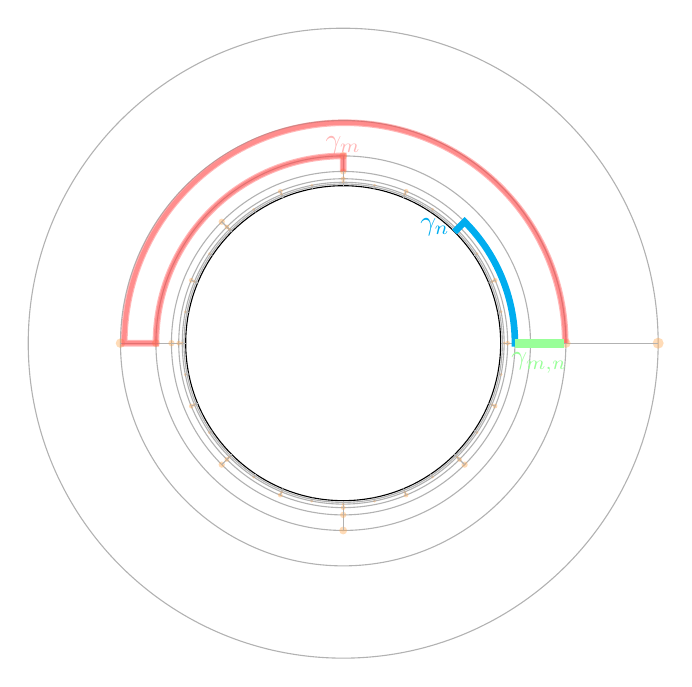
\begin{tikzpicture}[scale=2.0]
		
		
		
% The circles C_n
\draw (0,0) circle (1);
\foreach \i in {1,(1.0/2),(1.0/4),(1.0/8), (1.0/16), (1.0/32), (1.0/64)}{
\draw[black!30!white] (0,0) circle (2^\i);
}
   
\foreach \j in {0,1,2,3,4,5}{
    \pgfmathsetmacro{\jtwo}{2.0^\j}
    \pgfmathsetmacro{\jthree}{(1.0/\jtwo)}
    \pgfmathsetmacro{\twopower}{2^\jthree}
    \foreach \angleone in {1,...,\jtwo}{
    \pgfmathsetmacro{\anglez}{360*\angleone}
    \pgfmathsetmacro{\size}{1-\j/7.0}
    \fill[orange!70!white] (\anglez * \jthree: \twopower) circle (\size pt)[opacity=0.4];
    \draw[black!30!white] (\anglez * \jthree: \twopower) -- (\anglez * \jthree: 1);	
    }
}	

\draw [red!70!white,-,
double=red!70!white,
double distance=4\pgflinewidth, opacity=0.4,
] (1.41,0) arc (0:180:1.4) -- (-1.189,0) arc (180:90:1.189) -- (0,1.0905)
node[midway, above] {$\gamma_m$};

\draw [cyan,-,
double=cyan,
double distance=4\pgflinewidth,
] (1.4,0) -- (1.0905,0) arc (0:45:1.0905) -- (45:1) 
node[midway, left] {$\gamma_{n}$};;;


\draw [green!40!white,-,
double=green!40!white,
double distance=6\pgflinewidth,
] (1.0905,0) -- (1.4,0)
node[midway, below] {$\gamma_{m,n}$};


		
\end{tikzpicture}
	
	\caption{The three parts of an itinerary $\eta$. The green path is  $\gamma _{m,n}$,  the cyan and magenta are $\gamma _m$ and $\gamma_n$.
	} \label{fig:Three-parts-of-eta}
\end{figure}

